\documentclass[conference]{IEEEtran}

% -- Packages --------------------------------------------------------------
\usepackage{amsmath,amssymb,bm}
\usepackage{graphicx}
\usepackage[caption=false]{subfig}
\usepackage{booktabs}
\usepackage{multirow}
\usepackage{array}
\usepackage{xcolor}
\usepackage{hyperref}
\usepackage{cleveref}

% -- Macros ----------------------------------------------------------------
\newcommand{\States}{\mathcal{S}}
\newcommand{\Actions}{\mathcal{A}}
\newcommand{\Obs}{\mathcal{O}}
\newcommand{\Trans}{T}
\newcommand{\Rew}{R}
\newcommand{\ObsFn}{Z}
\newcommand{\Disc}{\gamma}
\newcommand{\belief}{b}
\newcommand{\pf}{\hat{b}}
\newcommand{\block}{\mathbf{p}_{\text{blk}}}
\newcommand{\goal}{\mathbf{p}_{\text{goal}}}
\newcommand{\sigmaobs}{\sigma_{\text{obs}}}
\newcommand{\sigmaep}{\sigma_{\text{ep}}}
\newcommand{\sdrift}{\sigma_{\text{drift}}}

% -- Title -----------------------------------------------------------------
\title{Belief-Augmented Reinforcement Learning for Pick-and-Place
       Under Observation Noise, Occlusion, and Target Drift}

\author{
  \IEEEauthorblockN{Allen Devaraj Augustin Ponraj}
  \IEEEauthorblockA{
    Department of Aerospace Engineering Sciences\\
    University of Colorado Boulder\\
    allendevaraj.augustinponraj@colorado.edu
  }
}

\begin{document}
\maketitle

% -- Abstract --------------------------------------------------------------
\begin{abstract}
Robotic pick-and-place under partial observability is challenging because
sensor noise, occlusion, and environmental disturbance corrupt or eliminate
target state information, turning a standard MDP into a POMDP.
This work formalizes the problem on a SO-ARM101 6-DOF arm in a physics-based
MuJoCo environment with three simultaneous uncertainty sources:
distance-dependent wrist-camera noise, occlusion by two distractor blocks,
and stochastic target drift ($\sdrift = 2$~mm/step).
Two learned policies are compared: plain PPO, which receives the raw (or
stale) wrist observation directly, and belief-augmented PPO, which routes
observations through a 300-particle bootstrap filter and exposes the filter
mean $\bm{\mu}$ and standard deviation $\bm{\sigma}$ to the policy.
A noise sweep across $\sigmaep \in \{3,\ldots,30\}$~mm reveals an unexpected
result: plain PPO achieves a flat $\sim\!82\%$ success rate independent of
noise level, indicating it learned a proximity-sweep strategy that bypasses
observation quality entirely.
Belief PPO achieves its largest advantage of $+11\%$ at $\sigmaep = 10$~mm,
where the particle filter converges reliably, but degrades to $-16\%$ at
$\sigmaep = 30$~mm as the filter operates outside its training distribution.
These results characterize the conditions under which belief augmentation
provides benefit, and expose a fundamental evaluation limitation:
proximity-based auto-grasp prevents the localization bottleneck from
manifesting at the task-success level.
\end{abstract}

% -- I. Introduction -------------------------------------------------------
\section{Introduction}
\label{sec:intro}

Robotic manipulation in unstructured environments requires reliable action
despite imperfect sensing.
Real wrist cameras return noisy pose estimates, distractor objects can
occlude the target, and physical perturbations shift objects between
observations.
Treating such settings as fully observable MDPs ignores fundamental epistemic
uncertainty and leads to brittle policies that degrade when sensor quality
changes or objects move unexpectedly.

This work studies a concrete instantiation: pick-and-place of a target LEGO
block in the presence of two occluding distractor blocks and stochastic
target drift, using only a wrist-mounted camera whose noise scales linearly
with end-effector-to-target distance.
Three uncertainty sources are active simultaneously.
\emph{Distance-dependent sensor noise:} the camera returns a
Gaussian-corrupted block pose; approaching improves observations, creating
an implicit information-gathering incentive.
\emph{Occlusion:} when a distractor interposes between camera and target,
the observation drops out entirely; the agent must reason from its last
known estimate.
\emph{Target drift:} the block undergoes random XY perturbations
($\sdrift = 2$~mm/step) while not held, so even a recent accurate estimate
decays as time passes.

Together these create a genuine exploration--exploitation tension in the
POMDP sense: at each step the agent chooses between spending more steps
refining its belief (approach for a better reading, reposition to clear
occlusion) and committing to a grasp on its current, imperfect estimate.
This mirrors the bandit arm-selection problem: each ``pull'' (approach
step) reduces the uncertainty about the block's position, but each step
also consumes horizon budget and risks triggering an incorrect auto-grasp.
The optimal policy must balance these competing pressures, a decision that
depends on the current belief uncertainty $\bm{\sigma}$ and how much
remaining budget is available.

Two learned policies are compared.
\emph{Plain PPO}~\cite{schulman2017ppo} treats the POMDP as a memoryless
MDP, receiving the last visible wrist observation replayed during occlusion.
It has no explicit mechanism to reason about uncertainty.
\emph{Belief-augmented PPO} maintains a bootstrap particle
filter~\cite{gordon1993novel} over the target pose and feeds both the
filter mean and its uncertainty estimate directly into the policy network,
enabling explicit uncertainty-conditioned behavior without an external
memory or recurrent architecture.

The main finding is that plain PPO learned to bypass the observation
entirely via a proximity-sweep strategy, achieving noise-invariant
performance across all tested levels.
Belief PPO is genuinely observation-dependent, outperforms at moderate
noise ($+11\%$ at $\sigmaep = 10$~mm), but degrades at noise levels beyond
its training distribution where the particle filter cannot converge.

\textbf{Departures from the proposal.}
The original proposal specified two uncertainty sources; a third (target
drift) was added to increase task difficulty and validate belief tracking
under nonstationary targets, which is more representative of real-world
scenes.
The end-effector Cartesian position was removed from the observation vector
after identifying it as redundant with joint angles via forward kinematics;
this reduced dimensionality from 16D/19D to 13D/16D.
The expected finding---that belief PPO uniformly outperforms---did not hold;
the actual noise-regime-dependent result is the central empirical
contribution.

% -- II. Background and Related Work ---------------------------------------
\section{Background and Related Work}
\label{sec:background}

\textbf{POMDPs for robotic manipulation.}
The POMDP framework~\cite{kaelbling1998pomdp} provides the formal
foundation for sequential decision-making under state uncertainty.
Kaelbling et al.\ define the belief-state MDP reduction in which the
agent maintains a posterior over hidden states and acts on that
distribution, guaranteeing that a sufficiently expressive belief
representation yields an optimal policy.
In robotic manipulation, partial observability arises from sensor noise,
occlusion, and contact uncertainty.
Koval et al.~\cite{koval2015manifold} model contact-induced uncertainty as
belief-space transitions, enabling planning over pose distributions rather
than point estimates.
This work addresses the complementary case of visual uncertainty:
wrist-camera noise and occlusion in a non-contact approach phase.

\textbf{Belief-state representations.}
The bootstrap particle filter~\cite{gordon1993novel} approximates the
belief as a weighted set of samples and naturally handles arbitrary
non-Gaussian distributions, including the multimodal beliefs that arise
when a target has been occluded long enough to occupy any location in a
region.
Kalman-family filters (KF, EKF, UKF) are computationally cheaper but
require unimodal Gaussian beliefs---an assumption that breaks after
extended occlusion.
In this environment, the two distractor blocks can occlude the target
for 50+ consecutive steps, making the particle filter the appropriate
representation.

\textbf{Deep RL for manipulation.}
Proximal policy optimization~\cite{schulman2017ppo} is widely used for
continuous-action robotic control due to its stability and relative ease
of hyperparameter tuning.
Reward shaping is known to be both critical and dangerous: Ng
et al.~\cite{ng1999potential} prove that only potential-based shaping
preserves the set of optimal policies, while arbitrary dense rewards can
introduce spurious local optima that trap the agent.
This guarantee was the design basis for the approach and carry shaping
terms used here; five distinct reward-hacking exploits discovered during
development were each resolved by converting the offending term to a
potential-based or one-time milestone form.

\textbf{Online POMDP planning.}
Silver and Veness~\cite{silver2010pomcp} introduced POMCP, extending
Monte Carlo tree search to POMDPs by using particle filters as belief
representations within the tree.
Sunberg and Kochenderfer~\cite{sunberg2018pomcpow} extend this to
continuous observation spaces via double progressive widening (POMCPOW),
which prevents the search tree from blowing up on every distinct
observation.
POMCP and POMCPOW provide the theoretical upper bound for what an online
planner with direct simulator access could achieve on this task.

% -- III. Problem Formulation ----------------------------------------------
\section{Problem Formulation}
\label{sec:problem}

\subsection{POMDP Definition}

The task is formalized as a POMDP tuple
$(\States,\, \Actions,\, \Obs,\, \Trans,\, \ObsFn,\, \Rew,\, \Disc)$.

\textbf{State space $\States$.}
The full (partially hidden) system state is
\begin{equation}
  s = \bigl(\mathbf{q},\;\block,\;\mathbf{p}_{d_1},\;\mathbf{p}_{d_2},\;h\bigr),
  \label{eq:state}
\end{equation}
where $\mathbf{q}=[q_1,\ldots,q_5,g]\in\mathbb{R}^6$ contains the five arm
joint angles and the gripper state $g\in\{0,1\}$ (both \emph{fully
observed} via joint encoders); $\block=(x_b,y_b,\theta_b)\in\mathbb{R}^3$
is the target block pose in the world frame (\emph{hidden});
$\mathbf{p}_{d_1},\mathbf{p}_{d_2}\in\mathbb{R}^3$ are the distractor
block poses (\emph{hidden}); and $h\in\{0,1\}$ is a binary flag indicating
whether the target is currently gripped (\emph{observed}: determined
by proximity, not a sensor reading).

\textbf{Action space $\Actions$.}
Actions are continuous 4-vectors
\begin{equation}
  a = \bigl[\Delta x,\;\Delta y,\;\Delta z,\;g_{\text{cmd}}\bigr]\in\mathbb{R}^4,
\end{equation}
where $\Delta x,\Delta y,\Delta z\in[-0.02,0.02]$~m are Cartesian
end-effector deltas and $g_{\text{cmd}}\in[-1,1]$ is the gripper command.
The environment resolves joint angles internally via geometric inverse
kinematics; the policy operates entirely in Cartesian space and never
directly commands joints.
Grasping is proximity-triggered: when the EE enters a sphere of radius
$r_{\text{grasp}}=15$~mm around any block, that block is automatically
attached via a rigid position constraint.
The policy therefore controls approach and positioning, not the grasp
trigger directly.

\textbf{Observation space $\Obs$.}
The agent receives a partial observation
\begin{equation}
  o_t =
  \begin{cases}
    \bigl[\,\underbrace{\mathbf{q}}_{6},\;
           \underbrace{\hat{\block}^{\,xy\theta}}_{3},\;
           \underbrace{\goal}_{2},\;
           h,\;
           c\,\bigr]
      & \text{plain PPO,} \\[8pt]
    \bigl[\,\underbrace{\mathbf{q}}_{6},\;
           \underbrace{\bm{\mu}}_{3},\;
           \underbrace{\bm{\sigma}}_{3},\;
           \underbrace{\goal}_{2},\;
           h,\;
           c\,\bigr]
      & \text{belief PPO,}
  \end{cases}
  \label{eq:obs}
\end{equation}
giving $o_t\in\mathbb{R}^{13}$ or $\mathbb{R}^{16}$ respectively.
Here $\hat{\block}$ is the (stale/noisy) wrist-camera reading of the target
pose, or the particle filter mean $\bm{\mu}$ in belief mode;
$\bm{\sigma}\in\mathbb{R}^3$ is the per-dimension particle filter standard
deviation (belief mode only);
$\goal\in\mathbb{R}^2$ is the fixed goal position in the world frame; and
$c\in\{0,1\}$ is a binary flag that is 1 when the wrist camera is occluded.
The EE Cartesian position is intentionally omitted: it is a deterministic
function of $\mathbf{q}$ via forward kinematics and carries no additional
information.

\textbf{Transition model $\Trans$.}
State transitions are defined implicitly by the MuJoCo physics engine
(\texttt{mj\_step}, 10 substeps at $\Delta t=0.0005$~s each).
Robot joint angles update deterministically from the IK-resolved target.
When not held, the target block undergoes stochastic drift:
\begin{equation}
  \mathbf{p}^{xy}_{\text{blk},t+1} = \mathbf{p}^{xy}_{\text{blk},t} + \epsilon,
  \quad \epsilon\sim\mathcal{N}(\mathbf{0},\,\sdrift^2\mathbf{I}_2),
\end{equation}
with $\sdrift=2$~mm/step.
Distractor blocks remain stationary throughout the episode.

\textbf{Observation function $\ObsFn$.}
The wrist-camera model is
\begin{equation}
  P(o_t\mid s_t) =
  \begin{cases}
    \mathcal{N}\!\bigl(\mathbf{p}^{xy\theta}_{\text{blk}},\;
      \Sigma_{\text{obs}}(d_t)\bigr)
      & \text{target visible,}\\[4pt]
    \delta(o_t - o_\tau)
      & \text{target occluded,}
  \end{cases}
  \label{eq:obs_fn}
\end{equation}
where
$\Sigma_{\text{obs}}(d_t)=\mathrm{diag}\!\bigl(\sigmaobs^2,\sigmaobs^2,
(10\sigmaobs)^2\bigr)$,
$\sigmaobs(d_t)=\max\!\bigl(\sigmaep,\;0.008\cdot(d_t/0.15)\bigr)$,
$d_t$ is the current EE-to-target distance, and $o_\tau$ is the last
visible reading replayed during occlusion.
The per-episode noise floor $\sigmaep\sim\mathcal{U}(3,15)$~mm is drawn
once at episode start and held fixed throughout.
Occlusion is determined geometrically: a frustum-based virtual wrist
camera with $25^\circ$ downward pitch and target-tracking yaw checks
whether any distractor's footprint projected onto the image plane
overlaps the target's footprint.

\textbf{Reward $\Rew$ and discount $\Disc$.}
The reward function is detailed in Table~\ref{tab:reward}.
The discount factor is $\Disc=0.99$ with a maximum episode horizon of
$T=300$ steps, after which the episode terminates as a timeout failure.

\subsection{Three Sources of Partial Observability}

Three distinct uncertainty sources make this task a genuine POMDP and
together produce the explore--exploit tension central to this work.

\textbf{1. Distance-dependent sensor noise.}
The effective observation standard deviation $\sigmaobs(d_t)$ grows with
distance, so the agent can actively reduce its own measurement uncertainty
by moving closer.
This creates a bandit-like incentive: approach more to localize better
before grasping (exploration), or commit to the current noisy estimate
(exploitation).
The optimal exploration depth is a function of the current belief
spread $\bm{\sigma}$, the inter-block spacing, and the remaining horizon.

\textbf{2. Occlusion-induced observation dropout.}
When a distractor interposes between the camera and the target, the
observation is completely absent for that step.
The agent cannot resolve this by approaching; it must reposition to
clear the distractor from the camera's line of sight.
Unlike sensor noise, occlusion uncertainty is \emph{not reducible by
approaching the target}---it requires a lateral repositioning maneuver
that may move the EE away from the target, trading off placement
progress for better information.
Per-step occlusion rates of $10$--$25\%$ are observed under trained
policies.

\textbf{3. Stochastic target drift.}
The target block drifts randomly by $\sdrift=2$~mm/step while ungripped,
making localization a moving-target problem.
A confident belief based on a reading taken $T_{\text{occ}}$ steps ago
has degraded by approximately $\sqrt{T_{\text{occ}}}\cdot\sdrift$ in
expected position error.
This third source was added over the original proposal to validate that
the particle filter's predict step can track a genuinely nonstationary
target; without drift, a simple last-observation cache is close to
optimal.

\subsection{Reward Function}

\begin{table}[!t]
  \caption{Reward function. Shaping rows marked $(\star)$ use
           potential-based form $w\cdot\mathrm{clip}(\Delta d/20\text{mm},{-1},1)$;
           bonus rows marked $(\dagger)$ fire once per episode on first entry.
           $d_{xy}$: EE-to-block XY distance. $d_g$: EE-to-goal distance.}
  \label{tab:reward}
  \centering
  \small
  \setlength{\tabcolsep}{5pt}
  \begin{tabular}{@{}l r l@{}}
    \toprule
    Component & Value & Trigger \\
    \midrule
    Step cost             & $-1.0$  & Every step \\
    XY approach$^{\star}$ & $\pm 3.0$ & Per step, pre-grasp \\
    Proximity bonus       & $\leq+2.0$ & $d_{xy}<25$~mm \\
    Close-in bonus        & $\leq+3.0$ & $d_{xy}<12$~mm \\
    Reach block$^{\dagger}$ & $+5.0$ & $d_{xy}<15$~mm \\
    Grasp target          & $+10.0$ & Correct block \\
    Grasp distractor      & $-15.0$ & Wrong block (terminates) \\
    Carry shaping$^{\star}$ & $\pm 5.0$ & Per step, while holding \\
    Near goal$^{\dagger}$ & $+5.0$  & $d_g<30$~mm, holding \\
    Perfect placement     & $+50.0$ & Release, $d_g<10$~mm \\
    Precise placement     & $+30.0$ & Release, $d_g<20$~mm \\
    Close placement       & $+10.0$ & Release, $d_g<40$~mm \\
    Missed release        & $-10.0$ & Release, $d_g\ge40$~mm \\
    \bottomrule
  \end{tabular}
\end{table}

The approach shaping (rows 2--5) follows the potential-based form of
Ng et al.~\cite{ng1999potential}: rewarding the improvement in a scalar
potential rather than the absolute value ensures that lingering near the
block provides no benefit beyond the one-time reach milestone.
Without this design, early experiments found the agent farming per-step
proximity rewards by hovering above the block without grasping.
The carry phase (rows 8--9) uses the same pattern once the target is held.
Terminal rewards (rows 10--13) are large relative to shaping terms to
ensure the episodic objective dominates.

\subsection{Simulation Environment}

\begin{figure}[!t]
  \centering
  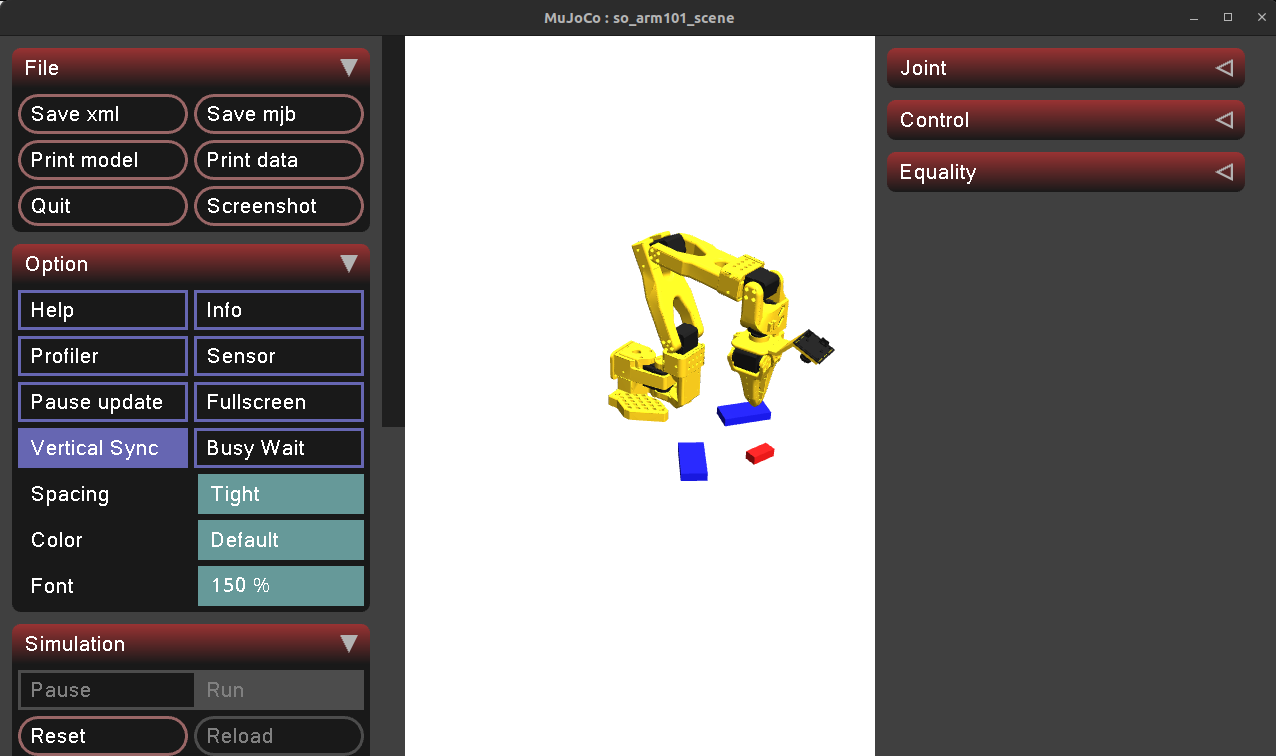
\includegraphics[width=0.85\columnwidth]{figs/mujoco_env_screenshot.png}
  \caption{MuJoCo simulation environment. The SO-ARM101 arm must grasp
           the red $2{\times}4$ LEGO target block and carry it to the
           yellow goal marker. Two taller blue $2{\times}2$ LEGO bricks
           serve as distractor/occluder objects, spawned within 90~mm of
           the target at each episode reset.}
  \label{fig:env}
\end{figure}

The SO-ARM101 is a 5-DOF desktop arm with a parallel-jaw gripper
(Fig.~\ref{fig:env}).
The MuJoCo scene contains a red $2{\times}4$ LEGO brick (target,
$32{\times}16$~mm footprint, $11$~mm tall), two blue $2{\times}2$ LEGO
bricks (distractors, $40{\times}20$~mm footprint, $33$~mm tall for
exaggerated wrist-camera occlusion), and a fixed yellow goal marker.
At each episode reset, the target is placed uniformly within the arm's
cylindrical reachable workspace ($r\in[12,22]$~cm, $\pm1$~rad from front);
distractors spawn uniformly within $90$~mm of the target with a minimum
$50$~mm inter-block separation.
The goal is sampled at least $100$~mm from any block.
The virtual wrist camera is co-located with the EE, pointed at the target
with a fixed $25^\circ$ downward pitch; its yaw tracks the target so that
the target is always inside the frustum when not occluded.

% -- IV. Solution Approach -------------------------------------------------
\section{Solution Approach}
\label{sec:approach}

\begin{figure*}[!t]
  \centering
  
\includegraphics[width=0.88\textwidth]{figs/system_pipeline.pdf}
  \caption{Architecture comparison.
           (a)~Plain PPO exposes the noisy or stale wrist-camera reading
           as a 13-D vector directly to the MLP policy.
           (b)~Belief-augmented PPO routes each step's observation through
           a 300-particle bootstrap filter; the filter summary
           $(\bm{\mu},\bm{\sigma})$ augments the 16-D policy input, giving
           the network an explicit uncertainty signal it can condition on.}
  \label{fig:pipeline}
\end{figure*}

\subsection{Plain PPO Baseline}

The plain PPO agent treats the POMDP as a memoryless MDP: during
occlusion it receives the cached last-visible wrist observation $o_\tau$
as if it were the current reading.
The 13-dimensional observation is given by~\eqref{eq:obs} (plain case).
The policy is a two-layer MLP with 256 hidden units per layer and ReLU
activations, matching the SB3 default architecture.

Training uses Stable-Baselines3~\cite{raffin2021sb3} PPO with
$n_{\text{env}}=8$ parallel environments (SubprocVecEnv),
$n_{\text{steps}}=4096$ per rollout, mini-batch size $256$,
$n_{\text{epochs}}=10$, entropy coefficient $0.02$,
$\gamma=0.99$, clip ratio $0.2$,
linearly-decayed learning rate $3\times10^{-4}\to 0$,
and VecNormalize applied to both observations and rewards
(clip threshold $\pm10$).
Training runs for $5\text{M}$ environment steps; an EvalCallback saves the
best checkpoint based on mean reward over 50 evaluation episodes every
10k training steps.

\subsection{Belief-Augmented PPO}

\subsubsection{Bootstrap Particle Filter}

A bootstrap (SIR) particle filter~\cite{gordon1993novel} maintains a
belief over the target's hidden pose
$\block=(x_b,y_b,\theta_b)$ using $N=300$ weighted particles
$\{x^{(i)}, w^{(i)}\}_{i=1}^N$.
The filter runs synchronously at each environment step.

\textbf{Predict.}
Each particle is perturbed to account for target drift and model
uncertainty:
\begin{equation}
  x^{(i)}_{t|t-1} = x^{(i)}_{t-1} + \epsilon,\quad
  \epsilon\sim\mathcal{N}\!\bigl(\mathbf{0},\,
    \mathrm{diag}(\sigma_p^2,\sigma_p^2,\sigma_{p\theta}^2)\bigr),
\end{equation}
with $\sigma_p=\max(0.5\text{ mm},\sdrift)=2$~mm and
$\sigma_{p\theta}=0.01$~rad.
Setting $\sigma_p\ge\sdrift$ ensures the filter's spread does not lag
behind the actual block drift.

\textbf{Update.}
When the target is visible ($c_t=0$), particle weights are updated by
the Gaussian likelihood:
\begin{equation}
  w^{(i)} \;\propto\; w^{(i)} \cdot
  \mathcal{N}\!\bigl(o_t^{xy};\;x^{(i)}_{xy},\;
    \sigma_{\text{lik}}^2\mathbf{I}\bigr),
  \quad \sigma_{\text{lik}} = 1.5\,\sigmaobs(d_t).
  \label{eq:pf_update}
\end{equation}
The $1.5\times$ likelihood widening prevents particle impoverishment:
using the exact sensor sigma collapses the effective sample size
$N_{\text{eff}}=1/\!\sum_i(w^{(i)})^2$ to near~1 each step, degenerating
the filter into a noisy running average.
During occlusion ($c_t=1$), the update step is skipped entirely;
particles spread via the predict step alone, correctly growing
$\bm{\sigma}$ without incorporating spurious information.

\textbf{Resample and reinject.}
Systematic resampling is applied when $N_{\text{eff}}<N/2$.
After resampling, $5\%$ of particles are re-injected near the last
visible observation to prevent degeneracy during extended occlusion.

\textbf{Belief summary.}
The filter output is compressed to
$(\bm{\mu},\bm{\sigma})\in\mathbb{R}^3\times\mathbb{R}^3$:
\begin{equation}
  \mu_k = \sum_i w^{(i)} x^{(i)}_k, \quad
  \sigma_k = \sqrt{\sum_i w^{(i)}\bigl(x^{(i)}_k - \mu_k\bigr)^2},
\end{equation}
for each dimension $k\in\{x,y,\theta\}$.
Large $\bm{\sigma}$ indicates recent or extended occlusion, or
accumulated drift uncertainty; small $\bm{\sigma}$ indicates confident
localization.

\subsubsection{Policy Architecture and Training}

The 16-dimensional belief observation is given by~\eqref{eq:obs}
(belief case).
The critical addition over plain PPO is $\bm{\sigma}$: the policy can
learn to act cautiously when uncertainty is high (slowing the approach
to avoid a wrong auto-grasp) and decisively when the filter is confident.
No explicit information-gathering reward is used; this uncertainty-aware
behavior must emerge from the task reward alone.

Reward shaping terms in belief PPO use the PF mean $\bm{\mu}$ in place
of the raw sensor reading when computing the approach distance gradient.
This provides a lower-variance reward signal at high noise levels, where
the raw observation can mislead shaping by several centimeters.
All PPO hyperparameters are identical to plain PPO; the network
architecture is the same MLP~[256,\,256].
The agent trains for $5\text{M}$ steps.

\begin{figure}[!t]
  \centering
  
\includegraphics[width=\columnwidth]{figs/belief_evolution.pdf}
  \caption{Belief $\sigma_{xy}$ (top) and EE-to-block distance (bottom)
           over a representative successful episode.
           Gray shaded spans mark wrist-camera occlusion windows.
           Uncertainty grows during each occlusion as particles spread via
           the predict step alone.
           Once occlusion clears and the agent approaches, $\sigma_{xy}$
           collapses rapidly as the distance-dependent noise model produces
           tight likelihoods at close range.
           The dashed green line marks the auto-grasp trigger.}
  \label{fig:belief-evo}
\end{figure}

% -- V. Results ------------------------------------------------------------
\section{Results}
\label{sec:results}

\subsection{Training Convergence}

\begin{figure}[!t]
  \centering
  \subfloat[Mean episode reward]{%
    
\includegraphics[width=0.48\columnwidth]{figs/learning_curves.pdf}%
  }
  \hfill
  \subfloat[Task success rate]{%
    
\includegraphics[width=0.48\columnwidth]{figs/success_curve.pdf}%
  }
  \caption{Training curves (15-step moving average).
           Dotted vertical lines mark the saved best-model checkpoints:
           plain PPO at $3.66$M steps (best reward $68.3$) and belief PPO
           at $3.25$M steps (best reward $71.7$).}
  \label{fig:learning}
\end{figure}

Training curves are shown in Fig.~\ref{fig:learning}.
Both agents discover the approach-shaping gradient around $1$M steps,
after which mean reward rises toward positive values.
Plain PPO reaches a peak mean reward of $68.3$ at step $3.66$M; belief PPO
achieves a slightly higher peak of $71.7$ at step $3.25$M, reflecting that
the particle filter provides a cleaner reward gradient through filtered
shaping.
All evaluations below use the saved best-model checkpoint rather than the
final checkpoint, which exhibits modest regression as the linear learning
rate schedule approaches zero.
Training variance is high throughout ($\pm130$ reward units) due to the
bimodal return distribution: successful episodes yield $+60$--$+100$,
while wrong-block grasps terminate early at approximately $-250$.

\subsection{Noise Sweep: Main Result}

\begin{figure}[!t]
  \centering
  \subfloat[Success rate vs.\ $\sigmaep$]{%
    
\includegraphics[width=0.48\columnwidth]{figs/noise_sweep.pdf}%
  }
  \hfill
  \subfloat[Belief $-$ Plain advantage]{%
    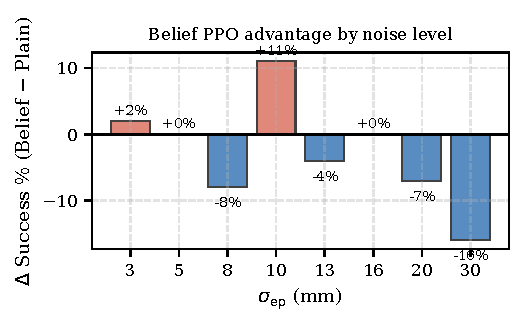
\includegraphics[width=0.48\columnwidth]{figs/noise_delta.pdf}%
  }
  \caption{Noise sweep results over 100 episodes per level (seed~42).
           Left: absolute success rates; the vertical dashed line marks
           the training maximum ($\sigmaep=15$~mm).
           Right: per-level advantage of belief over plain PPO.}
  \label{fig:noise_sweep}
\end{figure}

\begin{table}[!t]
  \caption{Noise sweep results (100 episodes, seed 42).
           \textbf{Bold} = higher success rate. $\Delta$ = Belief $-$ Plain.}
  \label{tab:noise_sweep}
  \centering
  \small
  \setlength{\tabcolsep}{4pt}
  \begin{tabular}{@{}c r r r r r@{}}
    \toprule
    \multirow{2}{*}{$\sigmaep$ (mm)}
      & \multicolumn{3}{c}{Success (\%)$\uparrow$}
      & \multicolumn{2}{c}{Mean ep.\ len.} \\
    \cmidrule(lr){2-4}\cmidrule(lr){5-6}
      & Plain & Belief & $\Delta$
      & Plain & Belief \\
    \midrule
    3  & \textbf{80} & 82          & $+2$            & 76.2  & 69.9  \\
    5  & 83          & \textbf{83} & $\phantom{+}0$  & 65.3  & 70.2  \\
    8  & \textbf{84} & 76          & $-8$            & 65.2  & 85.0  \\
    10 & 79          & \textbf{90} & $\bm{+11}$      & 75.8  & 45.5  \\
    13 & \textbf{86} & 82          & $-4$            & 57.0  & 72.4  \\
    16 & \textbf{84} & \textbf{84} & $\phantom{+}0$  & 66.1  & 63.5  \\
    20 & \textbf{81} & 74          & $-7$            & 72.4  & 93.3  \\
    30 & \textbf{82} & 66          & $-16$           & 68.3  & 116.4 \\
    \bottomrule
  \end{tabular}
\end{table}

The best-model checkpoints are evaluated at eight noise levels with
100 episodes each.
Results are in Fig.~\ref{fig:noise_sweep} and Table~\ref{tab:noise_sweep}.

The most striking finding is that plain PPO achieves near-constant success
($79$--$86\%$) across all eight noise levels, including $\sigmaep=30$~mm,
which is twice the training maximum.
This noise-invariant behavior indicates the policy learned a
\emph{proximity-sweep strategy}: the potential-based approach reward guides
the EE into the block's approximate XY region, and the $15$~mm auto-grasp
threshold is large enough to trigger once the EE reaches that region,
regardless of how corrupted the observation was.
Accurate localization is simply not required when the grasp threshold
exceeds the typical residual position error under this reward structure.

Belief PPO exhibits the expected observation-dependent behavior.
At $\sigmaep=10$~mm, the particle filter converges to a low-error estimate
within a few visible steps, enabling a decisive approach (mean $45.5$ steps
vs.\ $75.8$ for plain PPO) and the largest advantage of $+11\%$.
At $\sigmaep=30$~mm, the filter operates far outside its training
distribution: the likelihood at $\sigma_{\text{lik}}=45$~mm is nearly
flat, particle weights barely update, and the cloud cannot concentrate.
The policy responds by extending its search (mean $116.4$ steps vs.\
$68.3$ for plain PPO), and success falls to $66\%$ vs.\ $82\%$.
Within the training range ($\sigmaep\le15$~mm), the two methods are
roughly comparable, with belief PPO winning or tying at five of the six
in-distribution noise levels.

Zero wrong-block grasps are recorded for either policy at any noise level;
the grasp rate and task success rate are identical to within measurement
noise throughout Table~\ref{tab:noise_sweep}.
This confirms that the performance bottleneck is entirely in the
\emph{pre-grasp navigation} phase: once any agent reaches the target block
to within $15$~mm, it always grasps the correct block and places it
successfully.
The discrimination and placement sub-tasks are effectively solved; all
remaining failures are navigation timeouts.

\subsection{Belief Tracking Behavior}

Fig.~\ref{fig:belief-evo} shows the particle filter in operation over a
representative successful episode.
During each occlusion window (gray shading), $\sigma_{xy}$ grows steadily
as the predict-only step spreads particles to account for accumulated
drift uncertainty.
When occlusion clears and the agent begins approaching, $\sigma_{xy}$
collapses rapidly: at close range, $\sigmaobs(d_t)$ is small, so the
Gaussian likelihood peaks sharply and quickly concentrates the particle
cloud.
The auto-grasp fires immediately after $\sigma_{xy}$ reaches a low value,
consistent with the policy having learned an implicit confidence threshold
below which it commits to the grasp.
This sequence---uncertainty growth during occlusion, rapid collapse on
approach, then decisive commitment---is the qualitatively correct
behavior for the explore--exploit trade-off in this POMDP.

% -- VI. Discussion and Conclusion -----------------------------------------
\section{Discussion and Conclusion}
\label{sec:conclusion}

The central finding of this work is that proximity-based auto-grasp
fundamentally changes what task success measures.
With a $15$~mm grasp threshold and potential-based approach shaping,
any policy that reaches the approximate block region will succeed,
regardless of how accurately it localized the block.
Plain PPO learned exactly this: a robust proximity-sweep that ignores
observation quality and achieves a flat success curve from
$\sigmaep=3$~mm to $\sigmaep=30$~mm.
This is not a failure of plain PPO---it found the optimal strategy for
the task as designed---but it reveals a benchmark design limitation:
if the grasp threshold is large relative to the localization error, the
POMDP structure does not show up in the task metric.

Belief PPO, by contrast, genuinely uses observations.
The correlation between $\sigmaep$ and episode length in
Table~\ref{tab:noise_sweep} (belief: $45.5$ to $116.4$ steps; plain:
$57$--$76$ steps with no trend) is behavioral evidence that the policy
conditions its commit decision on $\bm{\sigma}$: at high noise it
searches longer before committing, exactly as an uncertainty-aware agent
should.
The degradation at $\sigmaep=30$~mm is not a fundamental flaw in the
belief-augmented approach but a distribution-shift failure: the particle
filter was trained and tuned for $\sigmaep\le15$~mm, and the likelihood
widening factor ($1.5\times$) that prevents impoverishment in-distribution
becomes insufficient at twice the training noise level.
Extending the training noise range or using a noise-adaptive likelihood
width would address this.

Reward engineering was the dominant development cost.
Over 18 training runs, five classes of reward-hacking exploit were
identified and resolved.
In every case the exploit was enabled by a per-step reward for occupying
a desired state (near the block, gripper closed near block, near goal
while holding): the agent learned to enter the state and remain there.
The fix was always either a one-time milestone (fires only on the first
entry into the state per episode) or a potential-based shaping term
(rewards only the improvement, not the absolute value)~\cite{ng1999potential}.
The former eliminates indefinite state occupancy; the latter provides dense
gradient signal while preserving the optimal policy.

Several limitations remain.
The grasp check is two-dimensional (XY proximity only), a pragmatic
choice after multiple failed attempts with a full $3$D check: with a
$3$D condition, the approach reward provides no gradient for the $z$
descent phase, since the $3$D proximity signal is zero when hovering
directly above the block.
Real-robot evaluation via the existing ROS2 integration was begun but
not completed; sim-to-real gaps in the noise model and block drift
dynamics remain untested.
Future work should tighten the grasp threshold (e.g., $5$~mm) to force
accurate localization to be task-critical, which would expose the full
benefit of belief augmentation at the task-success level.
Curriculum-based noise annealing and a noise-adaptive likelihood width
are straightforward extensions that would improve out-of-distribution
belief PPO performance.

% -- VII. Contributions and Release ----------------------------------------
\section*{Contributions and Release}

This was a solo project.
The MuJoCo simulation environment was designed and built from scratch
(\texttt{lego\_pick\_env.py}), including the three-phase reward function,
the multi-block frustum occlusion model, proximity-triggered constraint
grasping, stochastic target drift, and the full VecNormalize training
pipeline.
The bootstrap particle filter (\texttt{particle\_filter.py}) was implemented
independently, including the predict/update/systematic-resample cycle,
particle reinjection, and the widened-likelihood impoverishment heuristic.
The geometric occlusion checker (\texttt{occlusion.py}), the analytical
geometric IK (\texttt{compute\_workspace.py}), and the noise-sweep
evaluation harness (\texttt{eval\_noise\_sweep.py}) were all implemented
from scratch.
The PPO algorithm itself is from Stable-Baselines3~\cite{raffin2021sb3};
the MuJoCo physics engine and the SO-ARM101 robot URDF are third-party
assets.

The authors grant permission for this report to be posted publicly.

% -- References ------------------------------------------------------------
\begin{thebibliography}{99}

\bibitem{kaelbling1998pomdp}
L.~P. Kaelbling, M.~L. Littman, and A.~R. Cassandra,
``Planning and acting in partially observable stochastic domains,''
\emph{Artificial Intelligence}, vol.~101, no.~1--2, pp.~99--134, 1998.

\bibitem{koval2015manifold}
M.~C. Koval, N.~S. Pollard, and S.~S. Srinivasa,
``Pre- and post-contact policy decomposition for planar contact manipulation
under uncertainty,''
\emph{Int'l J. Robotics Research}, vol.~35, no.~1--3, pp.~244--264, 2016.

\bibitem{gordon1993novel}
N.~J. Gordon, D.~J. Salmond, and A.~F.~M. Smith,
``Novel approach to nonlinear/non-Gaussian Bayesian state estimation,''
\emph{IEE Proc.\ Radar and Signal Processing}, vol.~140, no.~2,
pp.~107--113, 1993.

\bibitem{schulman2017ppo}
J.~Schulman, F.~Wolski, P.~Dhariwal, A.~Radford, and O.~Klimov,
``Proximal policy optimization algorithms,''
\emph{arXiv:1707.06347}, 2017.

\bibitem{ng1999potential}
A.~Y. Ng, D.~Harada, and S.~Russell,
``Policy invariance under reward transformations: Theory and application
to reward shaping,''
in \emph{Proc.\ ICML}, 1999.

\bibitem{silver2010pomcp}
D.~Silver and J.~Veness,
``Monte-Carlo planning in large POMDPs,''
in \emph{Advances in NeurIPS}, 2010.

\bibitem{sunberg2018pomcpow}
Z.~Sunberg and M.~Kochenderfer,
``Online algorithms for POMDPs with continuous state, action, and
observation spaces,''
in \emph{Proc.\ ICAPS}, 2018.

\bibitem{raffin2021sb3}
A.~Raffin, A.~Hill, A.~Gleave, A.~Kanervisto, M.~Ernestus, and N.~Dormann,
``Stable-Baselines3: Reliable reinforcement learning implementations,''
\emph{JMLR}, vol.~22, no.~268, pp.~1--8, 2021.

\end{thebibliography}

\end{document}
